\chapter{Outer Product}

The outer product is an expansion operation. 
Two vectors give a matrix containing the vectors' dimensions; 
the dimensions where the two vectors were having one dimension and transform it into two-dimension.


Let $x$ and $y$ be the vectors of length $n$ and $m$ respectively.

\vspace*{0.5 cm}
$x = 
\begin{bmatrix}
    x_0 \\    
    x_1 \\    
    \vdots \\
    x_n \\    
\end{bmatrix}
,\ y = 
\begin{bmatrix}
    y_0 \\    
    y_1 \\    
    \vdots \\
    y_n \\    
\end{bmatrix}
$

\begin{equation}
    A = x \otimes y^T
    \label{eq:org_outer_prod}
\end{equation}
Or
\begin{equation}
    A = x \otimes y^T + A
    \label{eq:outer_prod}
\end{equation}

\[
\begin{bmatrix}
    x_0 \\    
    x_1 \\    
    \vdots \\
    x_n \\    
\end{bmatrix}
\otimes 
\begin{bmatrix}
    y_0 &   y_1 &    \dots &   y_n
\end{bmatrix}
=
\begin{bmatrix}
    x_0 \times y_0  & x_0 \times y_1    & \dots     & x_0 \times y_n \\
    x_1 \times y_0  & x_1 \times y_1    & \dots     & x_1 \times y_n \\
    \vdots          & \vdots            & \ddots    & \vdots \\
    x_n \times y_0  & x_n \times y_1    & \dots     & x_n \times y_n \\
\end{bmatrix}
\]

Where $A$ is the resultant matrix of dimensions $n$ and $m$.

The routine \textbf{?ger} implements the equation \ref{eq:outer_prod}, 
so we are doing the same. Once we implement the operation for one layout, 
another layout found using the exact implementation by rearranging 
the inputs. For example, if the implementation uses the column-major 
layout, then the row-major can be obtained by taking the matrix's 
transpose or exchanging the vectors

Taking the transpose on the both side in equation \ref{eq:outer_prod}.
\[A^T = (x \otimes y^T + A)^T\]

Transpose on the matrix addition is distributive, so we get
\[A^T = (x \otimes y^T)^T + A^T\]

We can transpose inside the outer product, but the vectors exchange 
their position and transpose self-cancellation operation.

\begin{equation}
    A^T = y \otimes x^T + A^T
    \label{eq:outer_prod_trans}
\end{equation}

If $A$ is a column-major then $A^T$ is must be row-major and vice-versa.

\clearpage
\section{Calculating Number of Operations}

Using equation \ref{eq:org_outer_prod}, we fill the below table

\begin{table}[ht]
    \centering
    \begin{tabular}{|c|c|}
        \hline
        \textbf{Name} & \textbf{Number} \\
        \hline
        Multiplication & $n \times m$ \\
        \hline
        Addition & $0$ \\
        \hline
    \end{tabular}
\end{table}

Total Number of Operations $=$ Number of Multiplication $+$ Number of Addition

Total Number of Operations $= n \times m + 0$

Total Number of Operations $= n \times m$

\section{Algorithm}

\begin{figure}[htb]
    \centering
    \subfloat[\centering Block Diagram]{{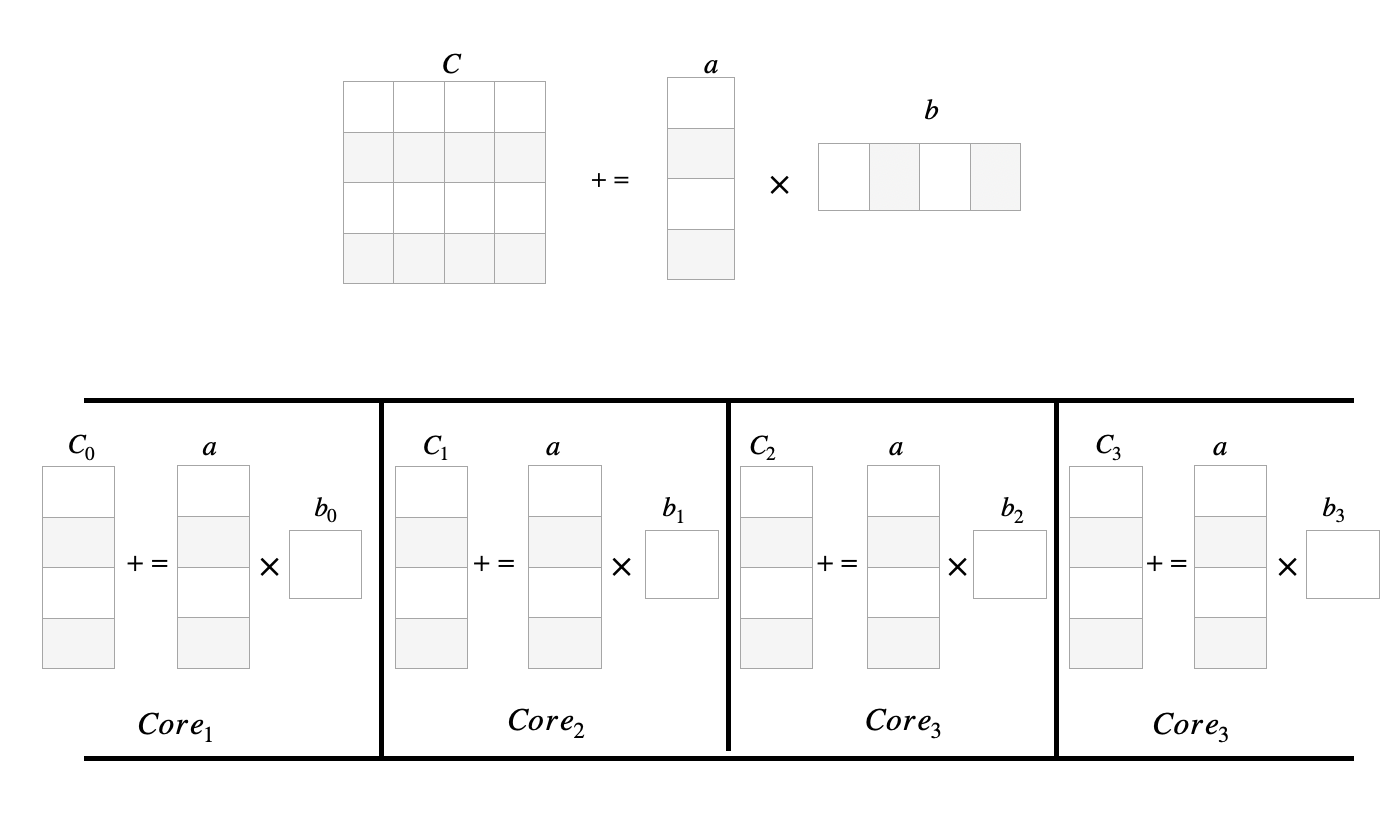
\includegraphics[width=10cm]{../assets/outer_product/Algo_visual.png} }}%
\end{figure}

\begin{algorithm}[H]
    \SetAlgoLined
    \SetKwFunction{SIMDFn}{outer\_simd\_loop}
    \SetKwProg{Fn}{Function}{:}{end}

    \tcp{$c$ is the pointer to the output matrix}
    \tcp{$a$ is the pointer to the first vector}
    \tcp{$b$ is the pointer to the second vector}
    \tcp{$n$ is the length of the vectors}
    \Fn{\SIMDFn($c$, $a$, $b$, $n$)}{
        \assignln{cst}{b[0]}

        \openmp{simd}
        \For{\assign{i}{0} \KwTo $n$ \KwBy 1}{
            \assignln{c[i]}{c[i] + a[i] \times cst}
        }
        \KwRet{$sum$}
    }
    \caption{Outer Product SIMD Function}
\end{algorithm}

\begin{algorithm}[H]
    \SetAlgoLined
    \KwIn{$c, wc, a, na, b, nb, max\_threads$}
    \tcp{$a$ and $b$ are vectors}
    \tcp{$c$ is the pointer to the output matrix}
    \tcp{$na$ is the size of the vector $a$}
    \tcp{$nb$ is the size of the vector $b$}
    \tcp{$wc$ is the leading dimension of the matrix $c$}
    \tcp{$max\_threads$ is the user provided thread count}
     \Begin{
        \assignln{MinSize}{256}
        \assignln{number\_el\_L_2}{\lfloor \frac{S_{L_2}}{S_{data}} \rfloor}
        \assignln{upper\_limit}{\lfloor \frac{number\_el\_L_2 - na}{na} \rfloor}
        \assignln{num\_threads}{max(1,min(upper\_limit,max\_threads))}
        $omp\_set\_num\_threads(num\_threads)$

        \openmp{parallel for if($nb$ $>$ $MinSize$)}
        \For{$i\gets 0$ \KwTo $ nb $ \KwBy $1$}{
            $aj \gets a$ \\
            $bj \gets b + i$ \\
            $cj \gets b + i \times wc $ \\
            $outer\_simd\_loop$($cj$, $aj$, $bj$, $na$)\\
        }
     }
    \caption{Vector-Vector Outer Product}
\end{algorithm}

Here, we start threads if the second vector's size exceeds $256$ because 
to avoid thread overhead for a small vector. The number is not concrete, 
so it can be any value until it small enough, or we can remove it. 
There is a problem we have to give a thought about and solve. 
This problem arises when multiple threads try to fetch the data, 
and if the data not found, it will evict the cached data using LRU policy. 
If the evicted data is still in use and it does not find the data will 
again evict and may or may not propagate to the other cores. 

To avoid the cache eviction problem, we decrease the threads spawned 
if the data cannot fit inside the cache.

Let the length of the first vector be $n$ and a small chunk of the second
vector be $m_c$.

$S_{L_2} = $ a block of matrix $+$ length of the first vector

We are not trying to fit the second vector because each core can 
put the element from the second vector inside the register and 
access each column of the resultant matrix and the whole first vector.
This algorithm is performing a rank-1 update in each core.

\begin{align*}
    S_{L_2} &= S_{data}(n \times m_c + n)\\
    n \times m_c &= \frac{S_{L_2}}{S_{data}} - n\\
\end{align*}

\begin{equation}
    m_c = \frac{S_{L_2}}{S_{data} \times n} - 1
    \label{eq:outer_block}
\end{equation}

As the $n$ increase, the block $m_c$ decreases. 
We control the second vector's blocks through the outer loop, 
where we divide the second vector through threads, and each 
thread contains a single element. Therefore, 
the $m_c$ block drops below the maximum allowed threads, 
we start to spawn $m_c$ amount of threads.

\begin{equation}
    num\_threads = max(1, min(m_c,max\_threads)) 
    \label{eq:outer_num_threads}
\end{equation}

\clearpage
\section{Performance Plots and Speedup Summary}

\begin{figure}[htb]
    \centering
    \caption*{Performance measurements of ?ger implementations}
    \subfloat[\centering Single-Precision]{{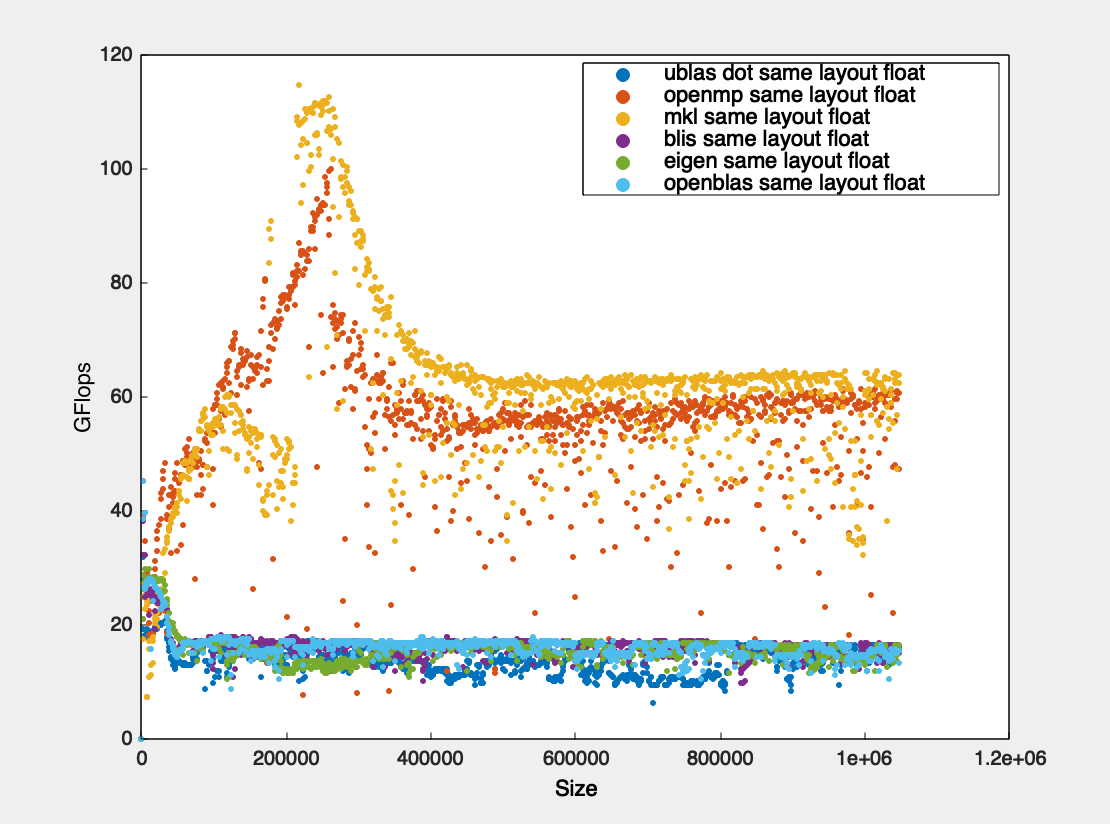
\includegraphics[width=8cm]{../assets/outer_product/float_GflopsVsSize.png} }}%
    \label{fig:outer_Sgflop220}
    \qquad
    \subfloat[\centering Double-Precision]{{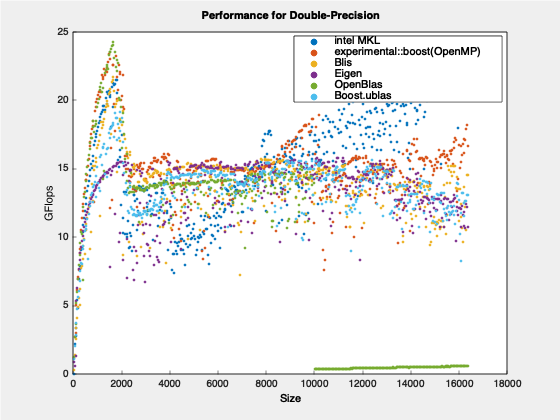
\includegraphics[width=8cm]{../assets/outer_product/double_GflopsVsSize.png} }}%
    \label{fig:outer_Dgflop220}
\end{figure}

\begin{figure}[htb]
    \centering
    \caption*{Sorted performance measurements of ?ger implementations}
    \subfloat[\centering Single-Precision]{{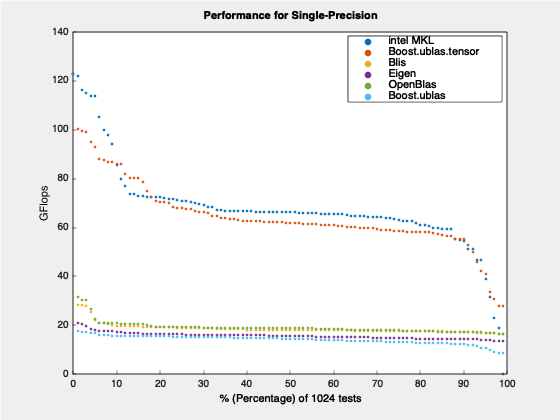
\includegraphics[width=8cm]{../assets/outer_product/float_GflopsVsSize_per.png} }}%
    \label{fig:outer_Sgflop_per220}
    \qquad
    \subfloat[\centering Double-Precision]{{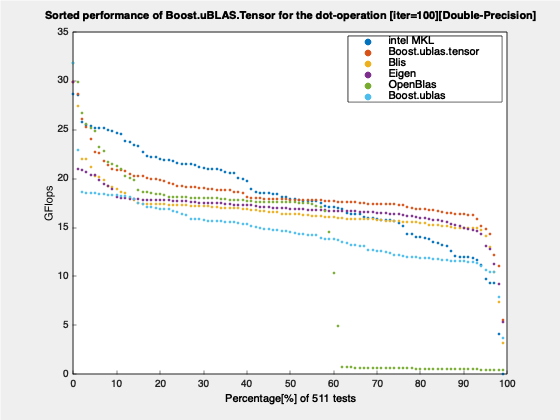
\includegraphics[width=8cm]{../assets/outer_product/double_GflopsVsSize_per.png} }}%
    \label{fig:outer_Dgflop_per220}
\end{figure}

\begin{figure}[htb]
    \centering
    \caption*{Comparison of the Boost.uBLAS.Tensor ?ger implementation}
    \subfloat[\centering Single-Precision]{{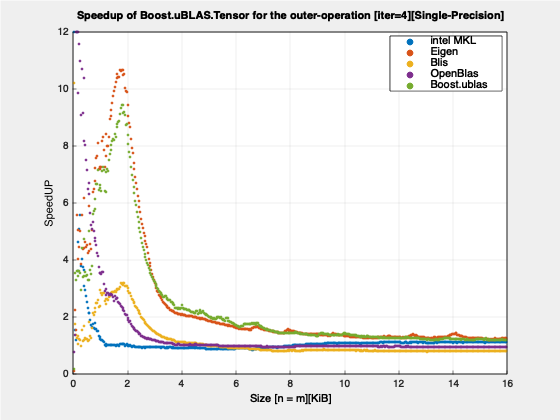
\includegraphics[width=8cm]{../assets/outer_product/float_Speedup.png} }}%
    \label{fig:outer_Sspeedup220}
    \qquad
    \subfloat[\centering Double-Precision]{{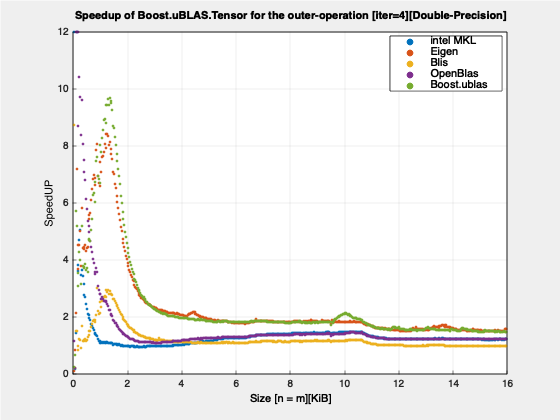
\includegraphics[width=8cm]{../assets/outer_product/double_Speedup.png} }}%
    \label{fig:outer_Dspeedup220}
\end{figure}

\begin{figure}[htb]
    \centering
    \caption*{Comparison of the Boost.uBLAS.Tensor ?ger implementation [semilogy]}
    \subfloat[\centering Single-Precision]{{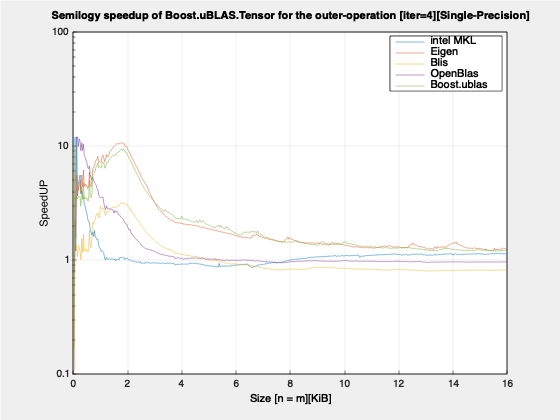
\includegraphics[width=8cm]{../assets/outer_product/float_Speedup_log10.png} }}%
    \label{fig:outer_Sspeedup_log10220}
    \qquad
    \subfloat[\centering Double-Precision]{{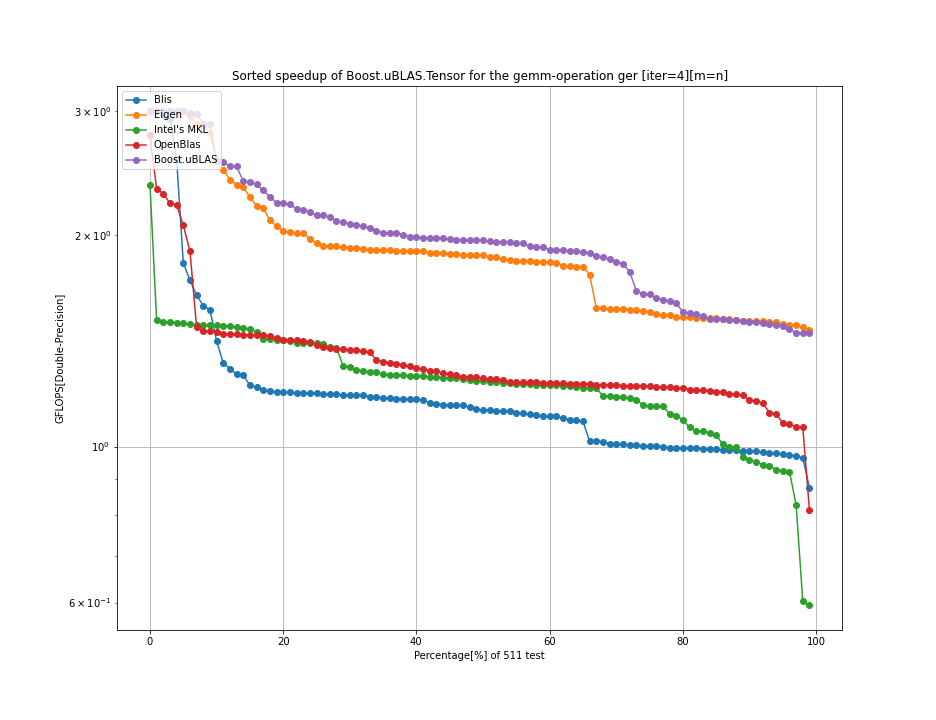
\includegraphics[width=8cm]{../assets/outer_product/double_Speedup_log10.png} }}%
    \label{fig:outer_Dspeedup_log10220}
\end{figure}

\begin{figure}[htb]
    \centering
    \caption*{Comparison of the Boost.uBLAS.Tensor ?ger implementation [sorted]}
    \subfloat[\centering Single-Precision]{{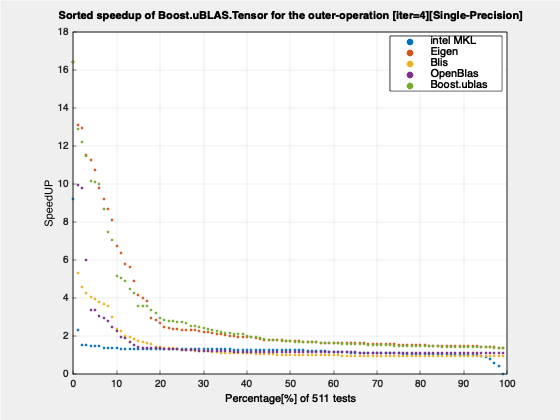
\includegraphics[width=8cm]{../assets/outer_product/float_Speedup_per.png} }}%
    \label{fig:outer_Sspeedup_per220}
    \qquad
    \subfloat[\centering Double-Precision]{{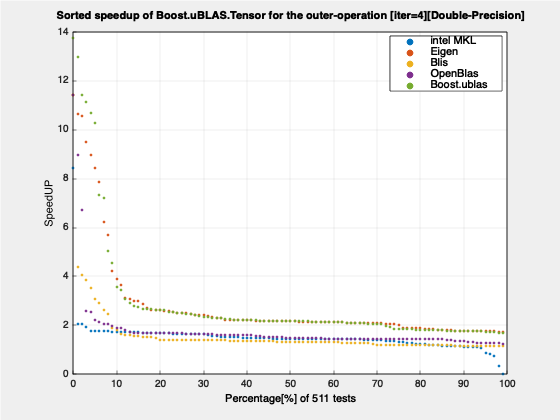
\includegraphics[width=8cm]{../assets/outer_product/double_Speedup_per.png} }}%
    \label{fig:outer_Dspeedup_per220}
\end{figure}

\begin{table}[ht]
    \centering
    \caption{Speedup Summary For Single-Precision}
    \begin{tabular}{|l|c|c|}
        \hline
        \textbf{Implementation} & \textbf{Speedup $\geq$ 1 [\%]} & \textbf{Speedup $\geq$ 2 [\%]}\\
        \hline
        Boost.uBLAS & $99$ & $34$ \\
        \hline
        OpenBLAS    & $99$ & $6$ \\
        \hline
        Eigen       & $99$ & $31$ \\
        \hline
        Blis        & $93$ & $8$ \\
        \hline
        Intel's MKL & $77$ & $0$ \\
        \hline
    \end{tabular}
    
    \begin{tabular}{|l|c|c|}
        \hline
        \textbf{Implementation} & \textbf{Speed-down $\geq$ 1 [\%]} & \textbf{Speed-down $\geq$ 2 [\%]}\\
        \hline
        Boost.uBLAS & $0$ & $0$ \\
        \hline
        OpenBLAS    & $0$ & $0$ \\
        \hline
        Eigen       & $0$ & $0$ \\
        \hline
        Blis        & $6$ & $0$ \\
        \hline
        Intel's MKL & $22$ & $1$ \\
        \hline
    \end{tabular}
    
    \vspace*{1 cm}

    \centering
    \caption{Speedup Summary For Double-Precision}
    \begin{tabular}{|l|c|c|}
        \hline
        \textbf{Implementation} & \textbf{Speedup $\geq$ 1 [\%]} & \textbf{Speedup $\geq$ 2 [\%]}\\
        \hline
        Boost.uBLAS & $99$ & $38$ \\
        \hline
        OpenBLAS    & $98$ & $5$ \\
        \hline
        Eigen       & $99$ & $23$ \\
        \hline
        Blis        & $76$ & $4$ \\
        \hline
        Intel's MKL & $86$ & $0$ \\
        \hline
    \end{tabular}
    
    \begin{tabular}{|l|c|c|}
        \hline
        \textbf{Implementation} & \textbf{Speed-down $\geq$ 1 [\%]} & \textbf{Speed-down $\geq$ 2 [\%]}\\
        \hline
        Boost.uBLAS & $0$ & $0$ \\
        \hline
        OpenBLAS    & $0$ & $0$ \\
        \hline
        Eigen       & $0$ & $0$ \\
        \hline
        Blis        & $22$ & $0$ \\
        \hline
        Intel's MKL & $13$ & $1$ \\
        \hline
    \end{tabular}
\end{table}

\clearpage
\section{Performance Metrics}

\subsection*{Range[Start: $32$, End: $16382$, Step: $32$]}

\begin{table}[ht]
    \centering
    \caption{GFLOPS For Single-Precision}
    \begin{tabular}{|l|c|c|}
        \hline
        \textbf{Implementation} & \textbf{Max} & \textbf{Average}\\
        \hline
        Boost.uBLAS.Tensor  & $35.316$ & $5.2823$ \\
        \hline
        Boost.uBLAS         & $2.48448$ & $1.8241$ \\
        \hline
        Intel's MKL         & $26.8859$ & $4.9064$ \\
        \hline
        OpenBLAS            & $13.4809$ & $3.2026$ \\
        \hline
        Blis                & $13.1177$ & $3.5963$ \\
        \hline
        Eigen               & $2.36464$ & $1.8591$ \\
        \hline
    \end{tabular}

    \vspace*{1 cm}

    \centering
    \caption{GFLOPS For Double-Precision}
    \begin{tabular}{|l|c|c|}
        \hline
        \textbf{Implementation} & \textbf{Max} & \textbf{Average}\\
        \hline
        Boost.uBLAS.Tensor  & $12.3296$ & $2.2376$ \\
        \hline
        Boost.uBLAS         & $1.21345$ & $0.9012$ \\
        \hline
        Intel's MKL         & $11.7715$ & $2.0042$ \\
        \hline
        OpenBLAS            & $7.00484$ & $1.5713$ \\
        \hline
        Blis                & $4.9330$ & $1.65328$ \\
        \hline
        Eigen               & $1.2312$ & $0.9391$ \\
        \hline
    \end{tabular}
\end{table}

\begin{table}[ht]
    \centering
    \caption{Utilization[\%] For Single-Precision}
    \begin{tabular}{|l|c|c|}
        \hline
        \textbf{Implementation} & \textbf{Max} & \textbf{Average}\\
        \hline
        Boost.uBLAS.Tensor  & $4.193$ & $0.627$ \\
        \hline
        Boost.uBLAS         & $0.294$ & $0.216$ \\
        \hline
        Intel's MKL         & $3.192$ & $0.582$ \\
        \hline
        OpenBLAS            & $1.600$ & $0.380$ \\
        \hline
        Blis                & $1.557$ & $0.427$ \\
        \hline
        Eigen               & $0.280$ & $0.220$ \\
        \hline
    \end{tabular}

    \vspace*{1 cm}

    \centering
    \caption{Utilization[\%] For Double-Precision}
    \begin{tabular}{|l|c|c|}
        \hline
        \textbf{Implementation} & \textbf{Max} & \textbf{Average}\\
        \hline
        Boost.uBLAS.Tensor  & $2.927$ & $0.531$ \\
        \hline
        Boost.uBLAS         & $0.288$ & $0.214$ \\
        \hline
        Intel's MKL         & $2.795$ & $0.475$ \\
        \hline
        OpenBLAS            & $1.663$ & $0.373$ \\
        \hline
        Blis                & $1.171$ & $0.392$ \\
        \hline
        Eigen               & $0.292$ & $0.223$ \\
        \hline
    \end{tabular}
\end{table}

\begin{table}[ht]
    \centering
    \caption{Speedup(Boost.uBLAS.Tensor) For Single-Precision}
    \begin{tabular}{|l|c|c|}
        \hline
        \textbf{Implementation} & \textbf{Max} & \textbf{Average}\\
        \hline
        Boost.uBLAS         & $14.2146$ & $2.895$ \\
        \hline
        Intel's MKL         & $1.3135$ & $1.0766$ \\
        \hline
        OpenBLAS            & $2.6197$ & $1.6493$ \\
        \hline
        Blis                & $2.6922$ & $1.4688$ \\
        \hline
        Eigen               & $14.9350$ & $2.8412$ \\
        \hline
    \end{tabular}

    \vspace*{1 cm}

    \centering
    \caption{Speedup(Boost.uBLAS.Tensor) For Double-Precision}
    \begin{tabular}{|l|c|c|}
        \hline
        \textbf{Implementation} & \textbf{Max} & \textbf{Average}\\
        \hline
        Boost.uBLAS         & $10.1607$ & $2.4827$ \\
        \hline
        Intel's MKL         & $1.0474$ & $1.1164$ \\
        \hline
        OpenBLAS            & $1.7601$ & $1.42407$ \\
        \hline
        Blis                & $2.4993$ & $1.3534$ \\
        \hline
        Eigen               & $10.014$ & $2.3827$ \\
        \hline
    \end{tabular}
\end{table}
